\section{Introduction}
System requirements and analysis provide a comprehensive overview of the essential components needed to design, build, and maintain the system successfully. This section covers the required hardware and software, browser compatibility difficulties, UI design criteria, and security procedures to ensure that the system functions properly while maintaining user satisfaction and data security.

\section{Project Perspective}
From a project perspective, the Asthma Disease Classification Using Machine Learning system aimed to classify asthma severity levels using data-driven techniques, assisting healthcare providers in making timely and accurate diagnoses. By building a robust pipeline that comprised data collection, preprocessing, feature engineering, model training, and deployment, this project made sure the solution was scalable, user-friendly, and reliable for real-world applications. This project demonstrated how machine learning may enhance healthcare process optimization, patient care, and medical decision-making.

\section{Project Function}
The Classification of Asthma Disease Based on patient data, a machine learning system is intended to provide medical practitioners with a sophisticated, dependable tool for determining the severity of asthma. The technology offers a thorough method to help physicians diagnose asthma more precisely and effectively by utilizing potent machine learning algorithms. To ensure a diversity of inputs for classification, the system gathers a range of patient data, such as demographics, medical history, spirometry results, and symptom frequency.


The system uses extensive data preprocessing procedures to guarantee the accuracy and dependability of the predictions. Imputation techniques are used to manage missing values, and inconsistencies are removed by normalizing numerical inputs to a standard range. Techniques like one-hot encoding are used to encode categorical variables, including symptom kinds or medication history, to make sure the data is in the right format for machine learning algorithms. Key clinical characteristics are the subject of feature selection and engineering procedures, which are essential for precise asthma severity prediction.

Based on their capacity to manage intricate, high-dimensional medical data, the machine learning models used in the system—Logistic Regression, Random Forest, and Support Vector Machines (SVM)—were carefully chosen. Accuracy, precision, recall, and F1-score are among the performance indicators used to assess each algorithm once it has been trained on historical data. Clinicians can evaluate the accuracy of the outcomes by using the confidence scores that the algorithm provides for each prediction. Clinical decision-making is facilitated by the visualization of these predictions through clear, simple charts and graphs.

Additionally, the system's deployment as an intuitive online application allows for seamless integration into clinical workflows. Through a secure web interface, medical personnel can immediately enter patient data, and the system provides immediate estimates of the severity of asthma. Comprehensive insights can be used to develop reports that support treatment planning and patient care. The web-based design of the system makes it simple to access from a variety of devices, such as smartphones, tablets, and desktop computers, enhancing the availability of vital diagnostic data across a range of healthcare environments.

Because the system manages sensitive patient data, security is a key component of the architecture. To protect patient privacy, all data exchanges are encrypted, and access control measures are put in place to guarantee that only individuals with the proper authorization can access and handle the data. To adhere to medical data regulations, regular security audits are conducted, guaranteeing the system's continued security and reliability.

In conclusion, by offering precise forecasts, real-time decision assistance, and secure data handling, the Asthma Disease Classification Using Machine Learning system not only improves the diagnostic skills of medical professionals but also raises the general effectiveness of asthma management. The system's user-friendly design and scalable architecture guarantee practical utility in actual medical settings, improving asthma treatment and results.



\section{General Constraint}
The limitations and conditions that must be taken into account when developing and implementing a system are referred to as general constraints. These restrictions ensure that the system operates effectively in the specified environment. Common constraints include hardware limitations that impact system performance, such as processor power, memory, or storage capacity. Additionally, software compatibility with specific operating systems or development tools may limit functionality. Time and resource constraints, including tight deadlines or budgetary constraints, may also have an effect on the project's scope. Additional restrictions may be imposed by legal and compliance requirements to safeguard data security and privacy, particularly in sensitive sectors like healthcare or finance. To provide a system that is scalable, dependable, and functional, these limitations must be recognized and addressed.
One of the main elements influencing a system's performance is frequently its hardware limitations. Particularly when working with big datasets or real-time processing, the hardware's processing power, memory, and storage capacity must be adequate to meet the application's computing demands. In the case of machine learning models, for example, insufficient hardware resources may lead to long training times, unsatisfactory model performance, or even system crashes. Delivering a high-performance application requires optimizing the system to function efficiently within the specified hardware constraints.
On the software side, limitations pertaining to the system's interoperability with particular operating systems or development platforms are frequently encountered. It may be necessary to modify the program or use certain libraries or frameworks in order for it to function flawlessly with the platforms and operating systems that end users will use. Furthermore, certain systems can be dependent on proprietary software or certain development tools, which could result in restrictions on their scalability, integration, or usefulness.

\section{Requirements}
\subsection{Hardware Requirements}The complexity of the system, including the amount of data it processes, the number of users accessing it at once, and the type of tasks it completes—especially for data analysis and machine learning—determines the hardware needs. The recommended hardware specifications are as follows:

\begin{itemize}
\item \textbf{Processor:} Minimum of Intel i5 or equivalent.
\item \textbf{RAM:} At least 4 GB for basic operations; 8 GB or more for smooth multitasking.
\item \textbf{Storage:} 2 GB of free disk space for browser-based usage and temporary storage.
\item \textbf{Browser Compatibility:} Browser-based and compatible with modern web browsers like Chrome, Firefox, Safari, or Edge.
\end{itemize}

\subsection{Software Requirements}
Supporting the system's development, implementation, and operation depends heavily on the software requirements. The platforms, frameworks, and tools listed below were utilized:

\begin{itemize}
\item \textbf{Operating System:} Windows 8 and above
\item \textbf{Code Language:} Python
\item \textbf{Tools:} Anaconda
\item \textbf{Editor:} Jupyter Notebook
\item \textbf{Libraries:} Numpy, pandas, sklearn, matplotlib, pickle, etc.
\end{itemize}

\section{Design}
To guarantee data integrity, model dependability, and defense against malevolent attacks, AI and ML systems need strong security measures. A condensed overview of important security procedures is provided below:


\begin{figure}[h]
\centering
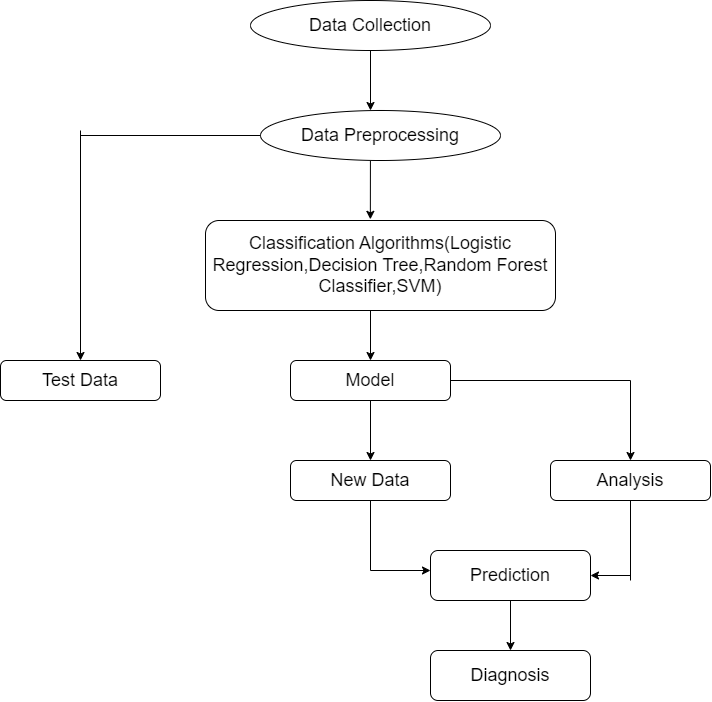
\includegraphics[width=0.7\linewidth]{Images/cc.png}
\caption{Context Flow Diagram}
\label{fig:enter-label}
\end{figure}

\begin{figure}[h]
\centering
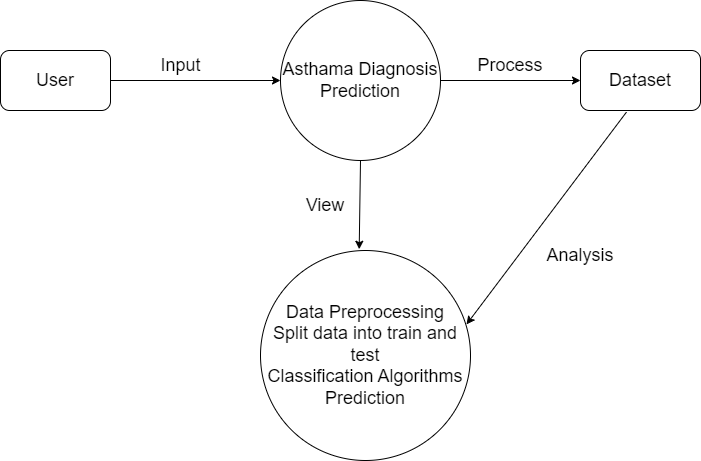
\includegraphics[width=0.7\linewidth]{Images/dd.png}
\caption{Data Flow Diagram}
\label{fig:enter-label}
\end{figure}
Data collection is a component of the asthma categorization system that entails gathering patient information such as demographics, symptoms, and medical history. To guarantee consistency, this raw data is cleaned and encoded during the data preprocessing step. The likelihood of asthma is then predicted using a variety of classification algorithms (such as SVM, Random Forest, Decision Tree, and Logistic Regression). The model processes fresh inputs to produce a prediction once its accuracy has been tested using different data. To guarantee a trustworthy diagnosis and assist well-informed healthcare decisions, the results are verified and examined.


The user, dataset, and processing components interact in the asthma diagnostic prediction system. A preloaded dataset containing patient data is used to process user inputs, such as symptoms. By separating data into training and testing sets, the system carries out data preprocessing. Predictions are produced using machine learning classification algorithms. An accurate diagnosis of asthma is aided by the analysis and display of these results to the user.
